% !TEX root = catron-dissertation.tex
\epstopdfsetup{outdir=./images/06_single_sensor_filtering/}

\chapter{Single Sensor Filtering Techniques}
\label{chap:06_single_filter}
\textcolor{red}{
  \begin{itemize}
    \item Work on the chapter intro
    \item Filter applied in Fourier space and multidimensional spectral space
  \end{itemize}
}

Transfer function, $H(j\omega) = H(s)$
Filter gain, $G(\omega) = |H(j\omega)|$
Filter phase, $\Phi(\omega) = \arg(H(j\omega))$
A filter is a function, $G(\mathbf{\omega})$, that describes the gain a signal will experience in frequency space.
In the simplest case, the filtered signal is the inverse Fourier transform of the gain multiplied by the Fourier transform of the signal.
Additionally, a windowing function, $W(\mathbf{x})$, can be used to help suppress finite sampling effects,
\begin{equation}
 f_F(\mathbf{x}) = \real\left(\ifftn[H(j\mathbf{\omega})\fftn\{\mathbf{x}\}]\right) \textrm{,}
 \label{eqn:06_filter_function}
\end{equation}
where $f$ is the signal function and $f_F$ is the filtered signal.
Depending on the windowing function some data could be destroyed during this process if there is a zero present due to the possibility of dividing by zero.

A basic MATLAB code for applying a filter to a wavefront using a separate function for both generating and applying the gain function which is presented in Listing \ref{code:sc_basic_wavefront_filters}.
This code generates a windowing function as described by Equations \ref{eqn:04_hann_window}, \ref{eqn:04_window_sep}, and \ref{eqn:04_window_space_arb}.
The temporal windowing function was generated with an additional two terms such that the end points which are equal to zero could be removed to prevent the first and last frames from being destroyed.
Likewise, the spatial window used the arbitrary aperture function which ensures that all of the points inside of the aperture are non-zero.
In some cases, a windowing function was not used due to filtered wavefront having a far greater magnitude in some places despite the precautions used.
The filter presented in this code sample is a second order temporal high-pass filter with a cutoff frequency of 2000 Hz.
The function \lstinline{WFfilter} takes input based on a normalized cut-point in reference to the sample rate.

\section{Temporal Filter Methods}
The methods presented in this section are based on Butterworth filters but could be extended to other types of filters.
The square of the transfer function of a Butterworth filter is \cite{Butterworth-1930-DvDrjKha},
\begin{equation}
 |H(j\omega)|^2 = G^2(\omega) = \frac{G_0^2}{1+\left(\frac{j\omega}{j\omega_c}\right)^{\pm2n}} \textrm{,}
 \label{eqn:06_butterworth}
\end{equation}
where $G_0$ is the zero-frequency gain, $\omega_c$ is the cutoff angular frequency, $n$ is the filter order (number of filters in a series), and $\pm$ represents either a low-pass ($+$) or high-pass ($-$) filter.
The gain of this filter is
\begin{equation}
  G(\omega) = \frac{G_0}{\sqrt{1+\left(\frac{\omega}{\omega_c}\right)^{\pm2n}}} \textrm{.}
  \label{eqn:06_butterworth_gain}
\end{equation}
A band-pass filter can be constructed by placing a low-pass in series with a high-pass filter and a band-stop by placing the two types in parallel.

In many tests, a large portion of the wavefront noise is at low frequencies primarily caused by mechanical vibration.
In general, a high-pass filter is useful in temporal space for removing this noise, since in many cases most of the power in the aero-optical signal occurs at higher frequency than the low-frequency mechanical vibration. as shown in Figure \ref{fig:06_filter_temporal}.
\begin{figure}
 \centering
 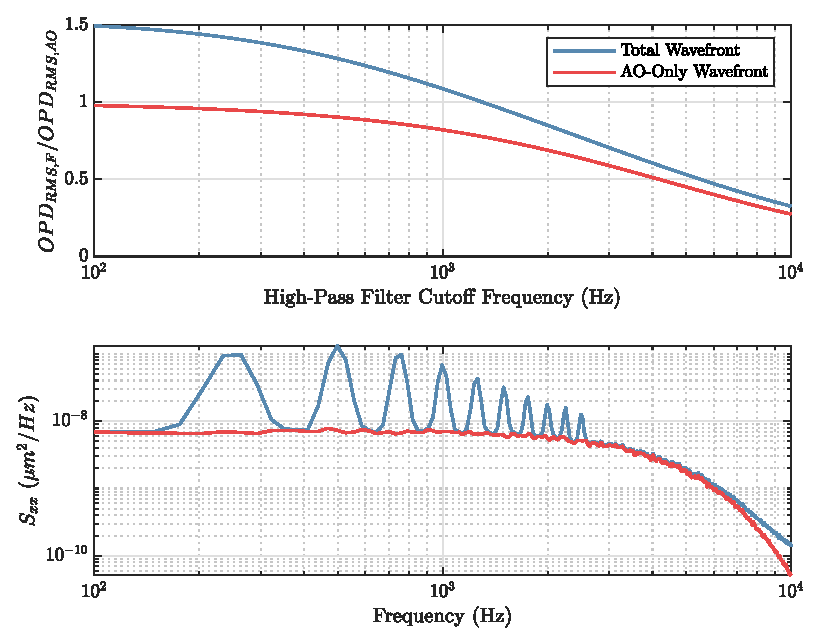
\includegraphics{../matlab/06_single_sensor_filtering/filter_temporal.eps}
 \caption{The $opdrms$ of high-pass temporal filtered wavefronts relative to the $opdrms$ of the aero-optical only unfiltered wavefront. Power spectra of both of the simulated wavefront versions.}
 \label{fig:06_filter_temporal}
\end{figure}
This figure shows the high-pass filtered $\opdrms$ of both the total and aero-optical only wavefronts high-pass filters with various cutoff frequencies, relative to that of the unfiltered $\opdrms$ aero-optical only wavefront.
Along with the filter performance plot is the power spectra of both of the simulated wavefront versions.
The results in Figure \ref{fig:06_filter_temporal} were computed for the synthetic wavefront created in Chapter \ref{chap:05_synthetic}.
The figure shows how a high-pass filter decreases the energy in the total wavefront and in the actual aero-optical wavefront, as the cutoff frequency increases.
The total wavefront ratio crosses unity around 1200 Hz, which is around the third harmonic of the blade-passing frequency in this simulated wavefront.
At this cutoff frequency ~75\% of the aero-optical signal remains and the remaining signal is made up by the remaining contamination.
This approach can provide a computationally inexpensive way of estimating the aero-optical portion of the wavefront for calculations that rely on the $\opdrms$ of a wavefront.
While it is more straightforward to determine a cutoff frequency for this synthetic wavefront since all of the signal components are fully known, a measured wavefront will likely take some knowledge or expectation of the contamination that is present in the measurement in order to select a high-pass filter cutoff frequency.

% \ref{tab:test}
% \begin{table}
% \centering
% \caption{Test Table}
% \input{../matlab/04_basic_filtering/filter_temporal.txt}
% \label{tab:test}
% \end{table}

An example of band-pass and band-stop filtering is shown in Figure \ref{fig:06_filter_temporal_bandpass}.
\begin{figure}
 \centering
 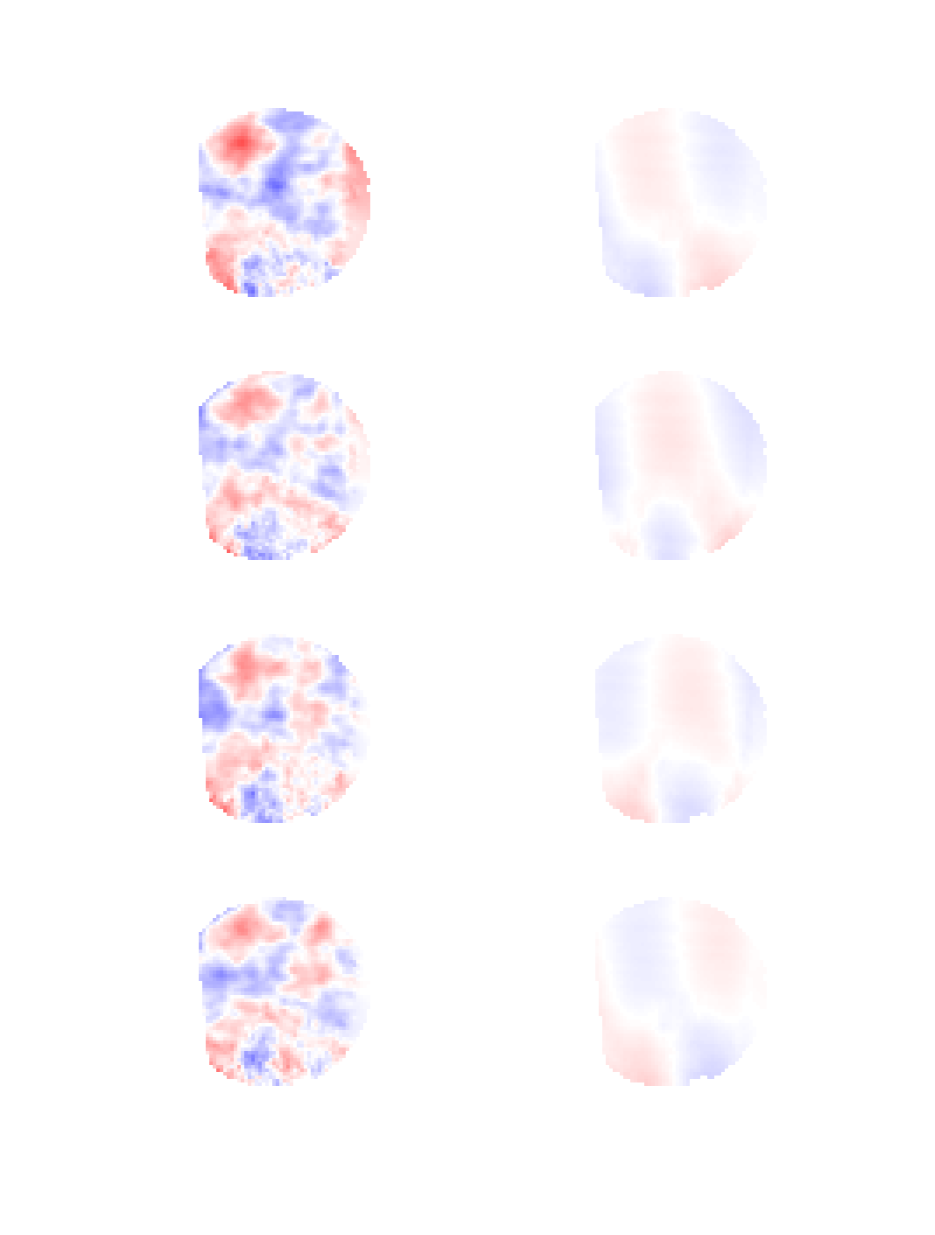
\includegraphics{../matlab/06_single_sensor_filtering/filter_temporal_bandpass.eps}
 \caption{Measured wavefronts filtered at the blade-passing frequency (532$\pm$10 Hz).  The left column is band-stop filtered while the right is band-pass filtered.}
 \label{fig:06_filter_temporal_bandpass}
\end{figure}
The figure shows several wavefront frames of the measured data presented in Chapter \ref{chap:03_optical_acoustics} in the Notre Dame White Field wind tunnel (see Figure \ref{ADD_REFERENCE}) that is band-stop filtered in the left column and band-pass filtered in the right column.
The flow is from right-to-left and the band-pass filtered wavefront clearly shows upstream-moving optical disturbances (moving left-to-right against the flow direction) associated with acoustic duct modes traveling upstream from the fan.
On the other hand, the band-stop filtered wavefronts on the left of Figure \ref{fig:06_filter_temporal_bandpass} show much slower-moving optical disturbances that are in general moving in the direction of the flow.
In particular, the downstream-moving disturbances on the left side of Figure \ref{fig:06_filter_temporal_bandpass} have the appearance of boundary-layer aero-optical disturbances, with a scale on the order of the boundary-layer thickness.

Note that for filters that operate in one-dimension, the filters were applied over both positive and negative frequencies to the n-dimensional Fourier transform in order to preserve the direction of travel of the signal.
This also allowed several filters to be applied in series with one another without having to perform a Fourier and inverse Fourier transform for each successive filter.
Temporal filters are also used in sizing and/or designing adaptive optics systems \cite{ADD_SOURCE} for example.
A low-pass filter with a cutoff at the bandwidth of either a fast-steering or deformable mirror is often used to define the signal that the system needs to reject \cite{ADD_SOURCE}.
A control system may need to have the bandwidth reduced in order to keep a mirror’s travel within limits \cite{ADD_SOURCE}, while a high-pass filter would inform designers of the remaining optical aberrations that cannot be corrected.



%Bookmark (page 53 of 4.3)
\section{Upstream/Downstream Moving}
In the preceding section, filters based on temporal frequency only were discussed. In this section, another filtering approach is presented in which signals are identified based on their dispersion velocity.
For the filtering of upstream and downstream moving optical disturbances a logistic function was chosen,
\begin{equation}
 f(x) = \frac{1}{1+\exp\{-kx\}} \textrm{.}
 \label{eqn:06_logistic}
\end{equation}
This function was then expanded into two-dimensions ($x$ and $t$) with the filter ideally returning a value of one in both the first and third quadrants and zero otherwise, for a filter that acts on disturbances moving in the direction of flow.
To accomplish this, the logistic curve in each dimension was scaled and offset to output values between negative one and positive one,
\begin{equation}
 G_t(f) = \frac{2}{1+\exp\{-k_tf\}}-1
 \label{eqn:06_logistic_time}
\end{equation}
and
\begin{equation}
 G_x(\xi_x) = \frac{2}{1+\exp\{\pm k_x\xi_x\}}-1 \textrm{,}
 \label{eqn:06_logistic_space}
\end{equation}
where $\pm$ determines whether the filter is designed to act on upstream-traveling disturbances ($+$) or downstream-traveling ($-$).
These two gain functions are then multiplied together and scaled to output values between zero and one,
\begin{equation}
 G(\xi_x,f) = \frac{(G_t\cdot G_x)+1}{2} \textrm{.}
 \label{eqn:06_up_down_filter}
\end{equation}
As the values of $k_x$ and $k_t$ go to infinity an ideal filter is obtained.
In a plot of the gain with the horizontal spatial frequency on the x-axis and the temporal frequency on the y-axis, an ideal filter for obtaining only the downstream traveling disturbances would have a gain of one in the first and third quadrants, zero in the second and fourth quadrants, and a value of $1/2$ when either frequency is zero.
The value of $1/2$ would equally split the component of a disturbance that is neither traveling upstream or downstream between the two directions.

The multidimensional spectrum using an ideal downstream moving filter on the synthetic wavefront is shown in Figure \ref{fig:06_filter_downstream} along side the dispersion of the unfiltered wavefront.
\begin{figure}
 \centering
 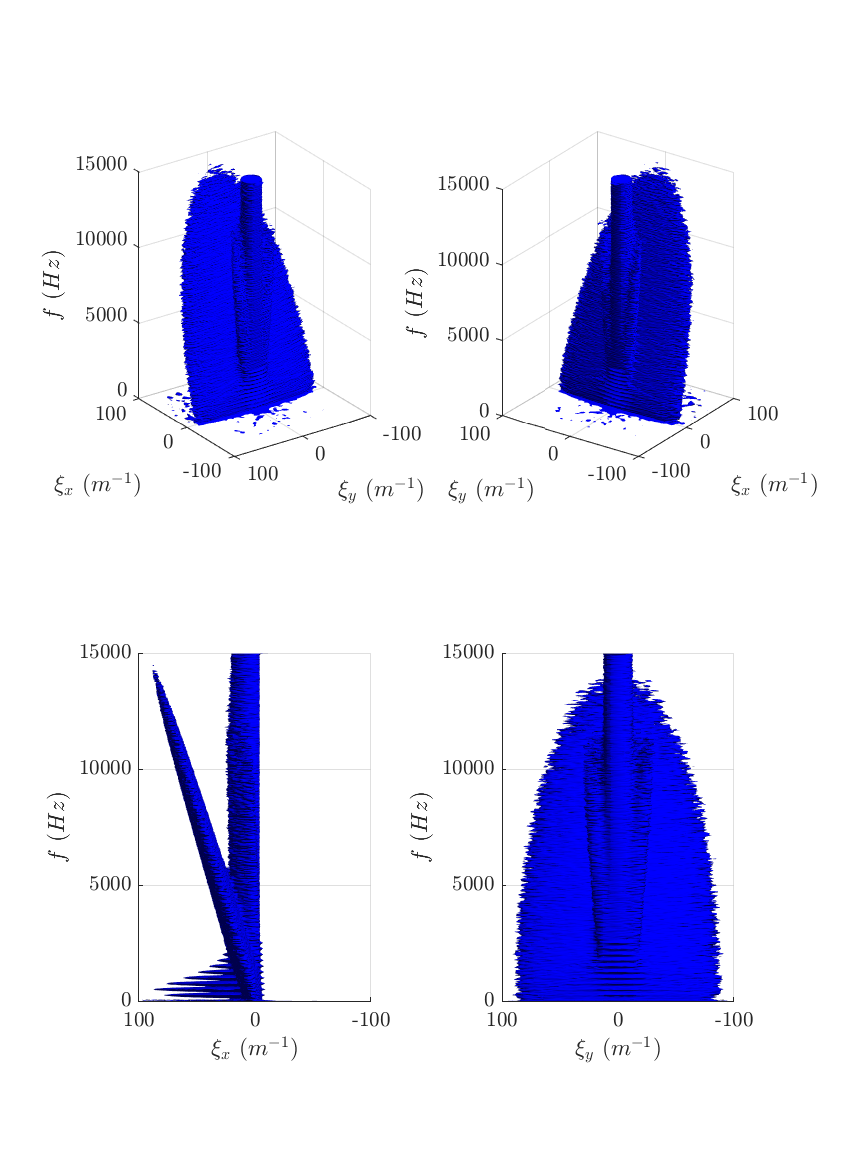
\includegraphics{../matlab/06_single_sensor_filtering/filter_downstream.eps}
 \caption{Multidimensional spectral isosurface of the synthetic wavefront with a downstream filter in place.}
 \label{fig:06_filter_downstream}
\end{figure}
All of the upstream traveling disturbances are removed and the disturbances at $\xi_x=0$ m$^{-1}$ are significantly reduced.
Some of the stationary modes remain while only the acoustic and vibration signals that are propagating in the direction of flow remain.
The aero-optical signal is clipped slightly at $\xi_x=0$ due to the spatial width of the signal.
The ratio of the time-averaged spatial-RMS of the filtered signal when compared to the aero-optical only signal was 1.24 while the unfiltered ratio was 1.53.
When the filter was applied to only the aero-optical signal the ratio was 0.96.
This filter method will retain any disturbance that is traveling in the direction of flow.
Even with an ideal filter there is some slight attenuation of the aero-optical signal due to signal having some spectral width that crosses into upstream-moving portion of the dispersion plot.


\section{Velocity Filtering}
Using dispersion analysis on a multidimensional spectral plot shows that flow structures traveling at a given speed as having a constant slope.
A plane in the multidimensional spectral plot can be used to measure a flow structure's velocity in both $x$ and $y$-directions.
The distance from any given point in the multidimensional spectral space to a plane described by the velocities $v_x$ and $v_y$ can be computed by
\begin{equation}
 d = \frac{|v_x\xi_x+v_y\xi_y-f|}{\sqrt{v_x^2+v_y^2+1}} \textrm{.}
 \label{eqn:06_dist_point_2_plane}
\end{equation}
Equation \ref{eqn:06_dist_point_2_plane} above can therefor be used to construct a low-pass or high-pass filter that retains only disturbances that are traveling at that velocity, or to exclude those disturbances respectively,
\begin{equation}
  G(d) = \frac{1}{\sqrt{1+\left(\frac{d}{d_c}\right)^{\pm2n}}} \textrm{.}
  \label{eqn:06_butterworth_velocity}
\end{equation}
where $d_c$ is the cutoff distance from the theoretical plane defined by the velocities $v_x$ and $v_y$.
Because of difference in the temporal and spatial sample rates of several orders of magnitude, the filter function used frequencies that have been normalized by the sample rate.


A low-pass velocity-filter of the synthetic wavefront is shown in Figure \ref{fig:06_filter_velocity}.
\begin{figure}
 \centering
 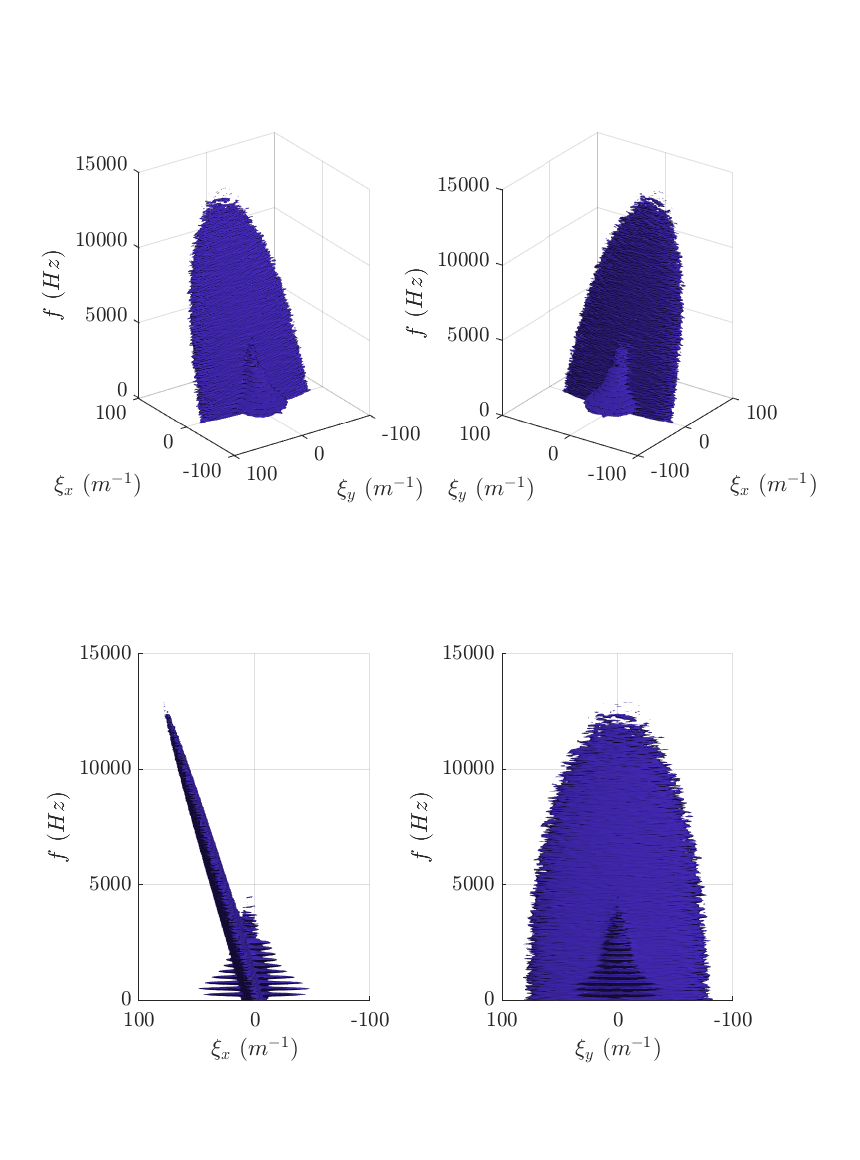
\includegraphics{../matlab/06_single_sensor_filtering/filter_velocity.eps}
 \caption{Multidimensional spectral isosurface of the synthetic wavefront with a low-pass velocity-filter in place.}
 \label{fig:06_filter_velocity}
\end{figure}
The filter was constructed for a $v_x$ at the mean boundary-layer velocity, $v_y$ of zero, $d_c$ of 1/80, and $n$ of 1.
The filtered multidimensional spectral plot shows primarily only the aero-optic signal remains with some additional low-frequency content from the blade-passing frequency and harmonic disturbances as well as some stationary and acoustic disturbances.
The ratio of the $\opdrms$ relative to that of the aero-optical only signal went from 1.53 in the unfiltered case to 1.01 in the filtered case.
This method can provide a very effective way to quickly estimate the $\opdrms$ of a convecting aero-optical disturbance in a noise-contaminated wavefront.

Another use of the velocity filter is measuring the speed of a broadband convecting disturbance such as the aero-optical signal of a boundary layer.
This can be accomplished by applying a series of low-pass velocity filters to the multidimensional spectrum of the wavefront along with a high-pass radial frequency filter to remove a significant portion of the stationary modes and acoustic cone,
\begin{equation}
  S_{xx,f}(\xi_x,\xi_y,f) = S_{xx}(\xi_x,\xi_y,f) G_v^2 G_\rho^2 \textrm{,}
\end{equation}
where $G_v$ is the velocity filter and $G_\rho$ is the radial frequency filter.
Once the wavefront has been filtered in multidimensional spectral space, the total power remaining can be calculated,
\begin{equation}
  P = \sum (S_{xx,f}\prod{\overrightarrow{f_s}}) \textrm{.}
\end{equation}
The average convective velocity of the structure will be the maximum power output.

This velocity finding procedure was tested on the synthetic wavefront which had a known boundary-layer mean velocity in Figure \ref{fig:06_filter_velocity_measure}.
\begin{figure}
 \centering
 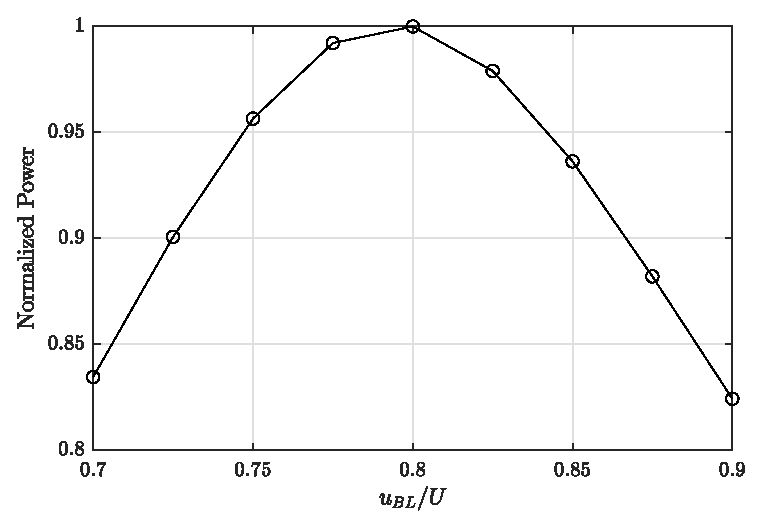
\includegraphics{../matlab/06_single_sensor_filtering/filter_velocity_measure.eps}
 \caption{Boundary layer velocity measurement of the synthetic wavefront using a combination of a low-pass velocity filter and a high-pass radial frequency filter. The maximum value at $u_{BL}/U=0.8$ corresponds with the actual value used in the creation of the synthetic wavefront.}
 \label{fig:06_filter_velocity_measure}
\end{figure}
The low-pass velocity filter used the same parameters as used previously except that $v_x$ was varied and the high-pass radial frequency filter used a cutoff value of 0.1 with an order of 2.
The radial frequency, $\xi_\rho=\sqrt{\xi_x^2+\xi_y^2}$, was normalized by the spatial sampling rate.
In this case boundary layer speed was determined to be 163 m/s which corresponds to the design velocity of the synthetic signal of $0.8U$.
For signals where the mean-velocity component that is not aligned with either the horizontal or vertical axis, both velocity components can be varied as shown in Figure \ref{fig:06_filter_velocity_real}.
\begin{figure}
 \centering
 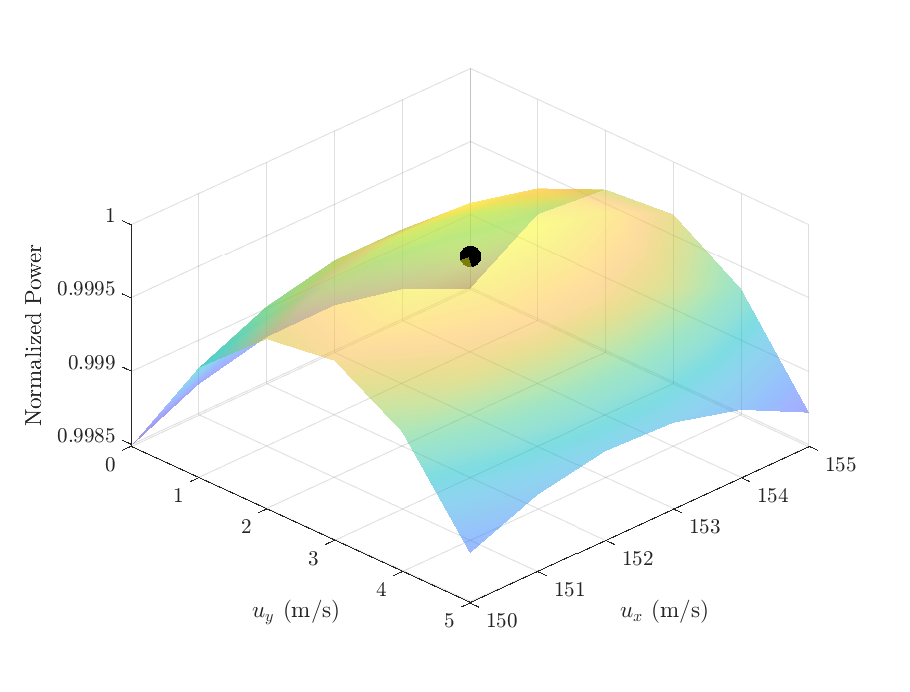
\includegraphics{../matlab/06_single_sensor_filtering/filter_velocity_real.eps}
 \caption{Velocity low-pass filter used to determine the mean disturbance velocity of measured data presented in Figure \ref{fig:04_dispersion_3d}.  The velocity in the x-direction was measured to be 207 m/s and -17 m/s in the y-direction.}
 \label{fig:06_filter_velocity_real}
\end{figure}
In this case the same filtering parameters were used as the synthetic case except the distance cutoff was 1/40 and both $v_x$ and $v_y$ were variables.
The velocity was measured using the boundary-layer optical disturbances in the multidimensional spectral plot to be approximately 152 m/s in the x-direction and 3 m/s in the y-direction.
The boundary-layer velocity was approximately $0.85U$ when compared to the pitot probe measurement of the free-stream velocity and the overall flow angle of the boundary-layer was approximately $1.1^\circ$.

\section{Baseline Spectrum}


\begin{figure}
  \centering
  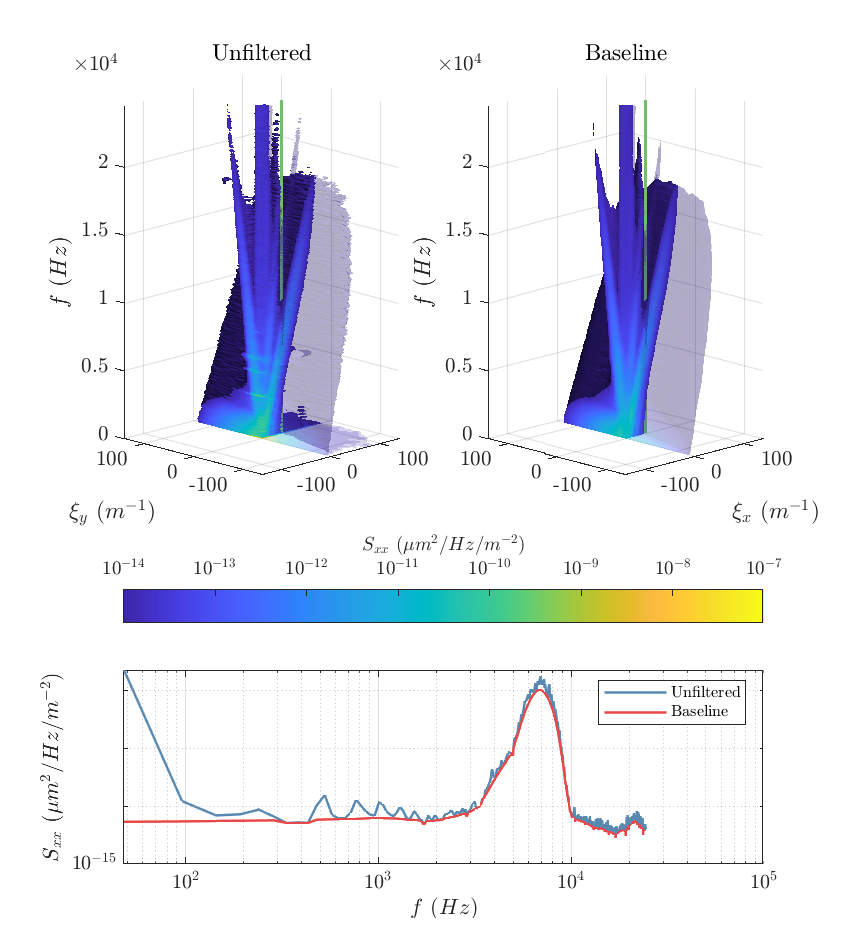
\includegraphics{../matlab/06_single_sensor_filtering/filter_baseline.eps}
  \caption{Baseline spectrum estimation.}
  \label{fig:06_filter_baseline}
\end{figure}




\section{Basic Filter Summary}
Three different basic wavefront filters were shown and discussed in this chapter.
The temporal filter is most useful when filtering out a frequency band of optical noise.
Besides filtering out optical noise, band-pass filters can be used to analyze a wavefront over a narrow-band to examine the optical aberrations at specific frequencies that significantly contribute to the overall optical disturbance; for example, as was shown in Chapter \ref{chap:03_optical_acoustics}, band-pass filters along with an implementation of an acoustic mode-marching method can help determine with some confidence that a narrow-band signal is likely to have been created by the wind-tunnel fan and can be removed.


Filters that separate upstream and downstream-moving disturbances are useful to filter out the optical contamination that comes from acoustic signals that are traveling upstream from a wind-tunnel fan.
These filters would also be useful for separating out an aero-optical signal that has a broad range of velocities that can occur in a span wise measurement of a boundary layer.
The velocity filter is the most useful for isolating the aero-optical portion of a wavefront measurement given the aero-optical signal has a fairly narrow and constant velocity range.
This filter also can be used to measure the speed associated with an optical disturbance in both x and y-directions.
